\documentclass{standalone}
\begin{document}

\section{Manipulating Sums}

Techniques for manipulating summations can often lead to a closed form solution or simpler summation.
This is especially helpful when dealing with multiple summations and loops in which the inner index depends on the outer.

\subsection{Basic Rules}

Often times a complex summation can be simplified using a few simple rules:

\begin{align*}
  &\sum_{k \in K} c a_k = c \sum_{k \in K} a_k &\text{Distribution} \\
  &\sum_{k \in K} (a_k + b_k) = \sum_{k \in K} a_k + \sum_{k \in K} b_k &\text{Association} \\
  &\sum_{k \in K} (a_k + b_k) = \sum_{p(k) \in K'} a_{p(k)} &\text{Commutativity}
\end{align*}

where $p(k)$ is a \emph{permutation} of the elements of $k$ to some set with image $p(k)$

For example, suppose $K  = \{-1, 0, 1\}$ and $p(k) = -k$, then $p : K \mapsto K'$ where $K' = \{1, 0, -1\}$.
The end result is the terms of $K$ are rearranged, and by \textbf{commutativity}, the summation is equal to the original ordering.

\subsubsection{Example}

Using the rules above, we can simplify the following summation:

\begin{align*} \label{eq:sum_manip_example}
  S &= \sum_{0 \leqslant k \leqslant n} (a + bk) \\
  &= a(n+1) + \sum_{0 \leqslant k \leqslant n} bk &\text{$a$ is constant} \\
  &= a(n+1) + \sum_{0 \leqslant n-k \leqslant n} bn - bk &\text{$k \to n-k$} \\
  &= a(n+1) + \sum_{0 \leqslant k \leqslant n} bn - bk &\text{$n-k \to k$} \\
\end{align*}

We employ another technique of adding $S$ to itself and solving a simplified expression

\begin{align*}
  2S &= \sum_{0 \leqslant k \leqslant n} (a + bk) + a(n+1) + \sum_{0 \leqslant k \leqslant n} bn - bk \\
  &= a(n+1) \sum_{0 \leqslant k \leqslant n} (an + bn) &\text{combining summations and simplifying} \\
  &= (n+1)(2a + bn) &\text{$an$, $bn$ constant}
\end{align*}

Finally, dividing by 2 we get $S = (a + \frac 1 2 bn)(n+1)$

\subsection{Iverson Notation}

In order to make manipulation of indexes easier, we can use notation invented
by Kenneth E. Iverson as an indicator function:

\begin{equation*} \label{eqn:iverson}
[P] =
\begin{cases}
  1 & \text{if $P$ is true} \\
  0 & \text{otherwise}
\end{cases}
\end{equation*}

\subsubsection{Properties}

Iverson brackets can be manipulated in the same way as set operations:

\begin{gather*}
  [P \land Q] = [P][Q] \\\\
  [P \lor Q] = [P] + [Q] - [P \cup Q] \\\\
  [\lnot P] = 1 - [P] \\\\
  [k \in A] + [k \in B] = [k \in A \cup B] + [k \in A \cap B] \\\\
  [k \in A \cap B] = [k \in A][k \in B]
\end{gather*}

\subsubsection{Example}

Using Iverson brackets, the "double-counting" summation identity can be derived
directly from the above properties.

\begin{equation*}
  [k \in K] + [k \in K'] = [k \in K \cap K'] + [k \in K \cup K']
\end{equation*}

which translates to summations with indices:

\begin{equation*}
  \sum_{k \in K} a_k + \sum_{k \in K'} a_k = \sum_{k \in k \cap K'} a_k + \sum_{k \in k \cup K'} a_k
\end{equation*}

\subsection{Perturbing the Sum}

Another technique is to manipulate the first and last terms. This reveal a way
to solve the summation via the above manipulations.

\subsubsection{Example}

For example, take the following summation representing a geometric series. A
good approach is to write $S_{n+1}$ in terms of $S_n$ and simplify the right
side of the equation.

Consider the following summation:

\[
  S_n = \sum_{0 \leqslant k \leqslant n} ax^k
\]

Adding the $n+1$st term and solving for $S_n$:

\begin{align*}
  S_n + ax^{n+1} &= a + \sum_{1 \leqslant k \leqslant n+1} ax^k \\
  &\iff S_n + ax^{n+1} = a + \sum_{1 \leqslant k+1 \leqslant n+1} ax^{k+1} \\
  &\iff S_n + ax^{n+1} = a + \sum_{0 \leqslant k \leqslant n} ax^{k+1} \\
  &\iff S_n + ax^{n+1} = a + xS_n \\
  &\iff S_n = \frac {a - ax^{n+1}} {1 - x}
\end{align*}

\subsubsection{Example}

Taking another example and using the results from the previous derivation, the
following sum is solved almost in the exact same way:

\[
  S_n = \sum_{0 \leqslant k \leqslant n} k2^k
\]

Once again perturbing the sum:

\begin{align*}
  S_n + (n+1)2^{n+1} &= 0 + \sum_{1 \leqslant k \leqslant n+1} k2^{k+1} \\\\
  &= \sum_{1 \leqslant k+1 \leqslant n+1} k2^{k+1} + \sum_{1 \leqslant k+1 \leqslant n+1} 2^{k+1} \\\\
  &= 2S_n + \sum_{0 \leqslant k \leqslant n} 2^{k+1}
\end{align*}

The second sum is a geometric series, and so after evaluating and simplifying:

\[
  S_n = \frac {2 - 2^{n+2}} {1 - 2} - (n+1)2^{n+1} = (n-1)2^{n+1} + 2
\]

\subsection{Multiple Sums}

When a summation is indexed by two or more indices, it can be written with more
than one sigma:

\[
  \sum_{1 \leqslant j, k \leqslant n} a_j b_k = \sum_{1 \leqslant j \leqslant n} \sum_{1 \leqslant k \leqslant n} b_k
\]

Summations of this form are evaulated "right-to-left" or by taking the "inner"
summtation first. In the above example, the summation over $k$ happens first.

\subsubsection{Interchanging Indices}

When indices are independent, this is simply a matter of rearranging the sums.
Complications arise when the inner index depends on the outer. The abstract way
of denoting an exchange of indicies:

\[
  \sum_j \sum_k a_{j,k} [P(j, k)] = \sum_{P(j,k)} a_{j,k} [P(j,k)] = \sum_k \sum_j a_{j,k} [P(j,k)]
\]

is a generalization of the associativity rule.

\subsubsection{Example}

This example shows how multiple summations can be split apart by applying the
associative rule and using Iverson notation.

Since the indices are independent, the summations can occur in either order.

\begin{align*}
  \sum_{1 \leqslant j,k \leqslant 3} a_j b_k
  &= \sum_{j,k} a_j b_k [1 \leqslant j \leqslant 3][1 \leqslant k \leqslant 3] \\
  &= \sum_j a_j [1 \leqslant j \leqslant 3] \sum_k b_k [1 \leqslant k \leqslant 3] \\
  &= \sum_{j=1}^3 a_j \sum_{k=1}^3 b_k
\end{align*}

\subsubsection{Harder Example}

In this example, $j$ is related to the value of $k$. Again, the problem can be
reduced into manipulating the inequalities using Iverson notation. Using the
following identity written in Iverson brackets:

\[
  [1 \leqslant j \leqslant n][j \leqslant k \leqslant n]
  = [1 \leqslant j,k \leqslant n]
  = [1 \leqslant k \leqslant n][1 \leqslant j \leqslant k]
\]

% TODO: Better tikz drawing

\begin{center}
  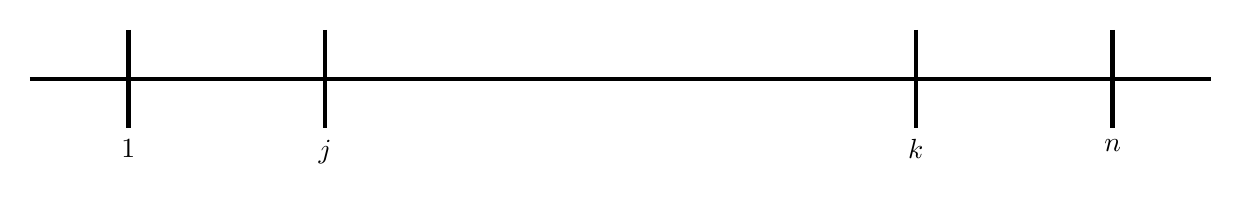
\begin{tikzpicture}[scale=2.5]
    \foreach \x/\y in {0/1, 1/j, 4/k, 5/n}
     \draw[ultra thick] (\x,0.25) -- (\x,-0.25) node[below]{$\y$};
    \draw[ultra thick] (-0.5,0)--(5.5,0);
  \end{tikzpicture}
\end{center}

This holds by combining the first two brackets by writing their intersection as
one inequality and by splitting it apart again.

An equivalent double summation can be manipulated using the above identity:

\begin{align*}
  \sum_{1 \leqslant j \leqslant n} \sum_{j \leqslant k \leqslant n} a_{j,k}
  &= \sum_{1 \leqslant j,k \leqslant n} a_{j,k} \\\\
  &= \sum_{1 \leqslant k \leqslant n} \sum_{1 \leqslant j \leqslant k} a_{j,k} \\\\
  &= \sum_{k=1}^n \sum_{j=1}^k a_{j,k}
\end{align*}

Hopefully, the second summation turns out to be easier to evaluate.

\end{document}
